\section{Logarithmic Functions} \label{S:0.4.Logarithms}


\vspace*{-14 pt}
\framebox{\hspace*{3 pt}
\parbox{6.25 in}{\begin{goals}
\item How can we ``undo'' the effects of exponentiation?
\item How can we solve equations involving exponential expressions?
\end{goals}} \hspace*{3 pt}}


\begin{web}
\item
    \href{https://www.khanacademy.org/math/algebra2/logarithms-tutorial/logarithm_basics/v/logarithms}{Khan
    Playlist: Logarithm basics}
\item
    \href{https://www.khanacademy.org/math/algebra2/logarithms-tutorial/logarithm_properties}{Khan
    Playlist: Properties of logarithms}
\item
    \href{https://www.khanacademy.org/math/algebra2/logarithms-tutorial/natural_logarithm}{Khan
    Playlist: Natural logarithms}
\item
    \href{https://www.khanacademy.org/math/algebra2/exponential_and_logarithmic_func/logarithmic-equations/v/solving-logarithmic-equations_dup_1}{Khan
    Playlist: Solving logarithmic equations}
\end{web}

\nin \hrulefill


\subsection*{Introduction}

In section \ref{S:0.2.Exponentials} we studied exponential functions to model a
variety of different settings.  It is straightforward to verify that the graph of an
exponential function passes the ``horizontal line test'' described in section
\ref{S:0.3.Transformations}, and so we should expect exponential functions to have
corresponding inverse functions.  In this section we will define the \emph{logarithm} to
be the inverse function for an exponential.

% Your preview activity goes here
\begin{pa} \label{PA:0.4}
	Carbon-14 ($^{14}$C) is a radioactive isotope of carbon that occurs naturally in the Earth's atmosphere.  During photosynthesis, plants take in $^{14}$C along with other carbon 	isotopes, and the levels of  $^{14}$C in living plants are roughly the same as atmospheric levels.  Once a plant dies, it no longer takes in any additional  $^{14}$C.  Since  $^{14}$C in the dead plant decays at a predictable rate (the half-life of $^{14}$C is approximately 5,730 years), we can measure  $^{14}$C levels in dead plant matter to get an estimate on how long ago the plant 	died.
	Suppose that a plant has 0.02 milligrams of $^{14}$C when it dies.
\ba
	\item Write a function that represents the amount of $^{14}$C remaining in the plant after $t$ years.
	\item Complete the table for the amount of $^{14}$C remaining $t$ years after the death of the plant.
        \begin{center}
            \begin{tabular}[h!]{| l |c|c|c|c|c|c|c|c|}
                \hline
                t & 0 & 1 & 5 & 10 & 100 & 1000 & 2000 & 5730 \\ \hline
                $^{14}$C Level & 0.02 & & & & & & & \\ \hline
            \end{tabular}
        \end{center}
	\item Suppose our plant died sometime in the past.  If we find that there are 0.014 milligrams of $^{14}$C present in the plant now, estimate the age of the plant to within 50 years.
        \ea
\end{pa} \afterpa


\subsection*{Logarithms}

\begin{definition}
Let $b>0$ with $b\neq1$. The \textbf{logarithm of }$x$ \textbf{with base }$b$ is defined by
	\[
		\log_{b}x=y\qquad\mbox{if and only if}\qquad x=b^{y}.
	\]
The expression $\log_{b}x$ represents the power to which $b$ needs to be raised in order to get $x$.

Two frequently used logarithmic functions are $\log_{10}x$ (frequently written $\log x$) and the natural logarithm $\log_{e}x$ (frequently written $\ln x$).
\end{definition}

Note that we have specifically defined logarithms to be inverse functions for
exponentials. For instance, $\log_{10}{1000} = 3$, since $10^{3} = 1000$.  Logarithmic
functions give us a way to re-write exponential expressions and, more importantly, solve
equations involving variables in an exponent.

\subsection*{Properties of Logarithms}
Since logarithms and exponentials are inverse functions, many of the properties of
logarithmic functions can be deduced directly from the properties of exponential
functions.  For example, the domain of all logarithmic functions is $(0,\infty)$ and the
range of all logarithmic functions is $(-\infty,\infty)$ because those are the range and domain, respectively, of exponential functions.  Similarly, logarithmic functions have a vertical asymptote at $x = 0$ because exponential functions have a horizontal asymptote at $y = 0$.  

\begin{figure}[ht!]     
	\begin{center}         
		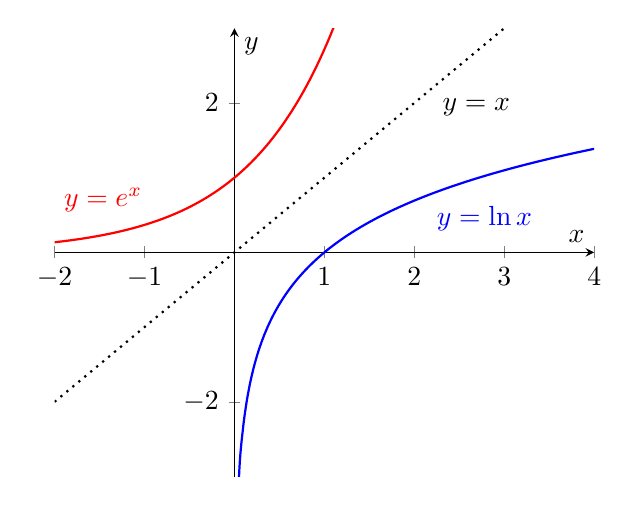
\begin{tikzpicture}[scale=1]             
			\begin{axis}[axis lines=center, xlabel={$x$}, ylabel={$y$}, domain=-2:4,
							ymin=-3, ymax=3,xmin=-2,xmax=4]
				\addplot[smooth, thick, blue, samples=150] {ln(x)}
						[below right] node[pos=0.75] {\color{blue}$y=\ln{x}$};
				\addplot[smooth, thick, red, samples=150] {exp(x)}
						[above left] node[pos=0.02] {\color{red}$y=e^{x}$};
				\addplot[smooth, black, dotted, thick] {x}
						[below right] node[pos=0.7] {\color{black}$y=x$};
			\end{axis}
		\end{tikzpicture}     
	\end{center}     
\caption{Graphs of the functions $y=e^{x}$ and $y=\ln{x}$.}     
\label{F:0.4.Ex1} 
\end{figure}

The following properties of logarithms can be deduced from the properties of exponential functions and the definition of the logarithm.  These properties are especially useful in simplifying or solving logarithmic and exponential equations.
\begin{callout}
    {\bf Properties of logarithms:} For $b>0$, $b \ne 1$, and $x,y>0$:
\begin{enumerate}
\item $\log_{b}1=0$
\item $\log_{b}b=1$
\item $\log_{b}\left(xy\right)=\log_{b}x+\log_{b}y$
\item $\log_{b}\left(\dfrac{x}{y}\right)=\log_{b}x-\log_{b}y$
\item $\log_{b}x^{r}=r\,\log_{b}x$
\item $\log_{b}b^{x}=x$
\item $b^{\log_{b}x}=x$
\item $\log_{b}x=\log_{b}y$ if and only if $x=y$
\end{enumerate}
\end{callout}


\begin{activity}\label{A:0.4.1}
    Use the definition of a logarithm along with the properties of logarithms to answer
    the following.
    \ba
\item Write the exponential expression $8^{1/3} = 2$ as a logarithmic expression.
\item Write the logarithmic expression $\log_2 \frac{1}{32} = -5$ as an exponential
    expression.
\item What value of $x$ solves the equation $\log_2 x = 3$?
\item What value of $x$ solves the equation $\log_2 4 = x$?
\item Use the laws of logarithms to rewrite the expression $\log \left( x^3 y^5 \right)$
    in a form with no logarithms of products, quotients, or powers.
\item Use the laws of logarithms to rewrite the expression $\log \left( \frac{x^{15}
    y^{20}}{z^4} \right)$
    in a form with no logarithms of products, quotients, or powers.
\item Rewrite the expression $\ln(8) + 5 \ln(x) + 15 \ln(x^2+8)$ as a single logarithm.
    \ea


\end{activity}
\begin{smallhint}
    Use the properties of logarithms.
\end{smallhint}
\begin{bighint}
    Use the properties of logarithms.
\end{bighint}
\begin{activitySolution}
    \ba
\item $8^{1/3} = 2$ is equivalent to $\log_8 2 = \frac{1}{3}$.
\item $\log_2 \frac{1}{32} = -5$ is equivalent to $2^{-5} = \frac{1}{32}$.
\item $\log_2 x = 3$ is equivalent to $x = 2^3 = 8$.
\item $\log_2 4 = x$ is equivalent to $2^x = 4$ and we see that $x=2$ since $2^2 = 4$.
\item Using the product and power properties
    \[ \log\left( x^3 y^5 \right) = 3\log(x) + 5\log(y). \]
\item Using the product, power, and quotient properties
    \[ \log\left( \frac{x^{15} y^{20}}{z^4} \right) = 15\log(x) + 20\log(y) - 4\log(z). \]
\item Using the power and product properties
    \[ \ln(8) + 5 \ln(x) + 15\ln(x^2+8) = \ln\left( 8 x^5 \left( x^2 + 8 \right)^{15}
        \right) \]
    \ea
\end{activitySolution}

\aftera



\bex
Find a value of $x$ for which $3^{x}=13$.
\eex
To isolate the variable $x$, we should take the logarithm of both sides. For convenience, let's choose to use the logarithm base 10.
	\[
		\log(3^{x})=\log(13).
	\]
Applying logarithm property (5), we find
	\[
		x\,\log3=\log13.
	\]
Solving algebraically for $x$ yields
	\[
		x=\frac{\log13}{\log3}\approx2.3347.
	\]
NOTE: Our choice to use the logarithm base 10 was arbitrary. We could have chosen any base for our logarithm to solve this equation.
% \afterex

\bex
In 1970, the population of the United States was approximately 205.1 million people. Since that time, the population has grown at an annual rate of approximately 1.05\%. Assuming that this growth rate continues, when would we expect the population of the United States to reach 350 million?
\eex
Since the rate of growth of the population is proportional to the size of the population, we should use an exponential model for this problem. That is, we want
	\[
		P(t)=P_{0}e^{rt}
	\]
where $t$ is the number of years after 1970, $P(t)$ is the population (in millions) of the United States at time $t$, $P_{0}$ is the population (in millions) of the United States in 1970 (i.e. $t=0$) and $r$ is the rate of growth of the population. To determine when the population will reach 350 million, we must solve the equation 
	\[
		350=205.1e^{0.0105t}.
	\]
To solve for $t$, we need to first solve for the exponential expression by itself and then use logarithms. Dividing both sides of the equation by 205.1 gives
	\[
		\frac{350}{205.1}=e^{0.0105t}.
	\]
Taking the natural logarithm of both sides gives
	\[
		\ln\left(\frac{350}{205.1}\right)=\ln\left(e^{0.0105t}\right).
	\]
Applying logarithm property (6), we find
	\[
		\ln\left(\frac{350}{205.1}\right)=0.0105t.
	\]
Finally, solving algebraically for $t$ gives
	\[
		t=\frac{1}{0.0105}\ln\left(\frac{350}{205.1}\right)\approx50.9\,\mbox{years}.
	\]
Thus, we expect the population of the United States to reach 350 million in 2021 (approximately 51 years after 1970).
\afterex

\begin{activity}\label{A:0.4.2}
    Solve each of the following equations for $t$, and verify your answers using a calculator.
	\ba
		\item $\ln t=4$
		\item $\ln(t+3)=4$
		\item $\ln(t+3)=\ln4$
		\item $\ln(t+3)+\ln(t)=\ln4$
		\item $e^{t}=4$
		\item $e^{t+3}=4$
		\item $2e^{t+3}=4$
		\item $2e^{3t+2}=3e^{t-1}$
	\ea

\end{activity}
\begin{smallhint}
    
\end{smallhint}
\begin{bighint}
    
\end{bighint}
\begin{activitySolution}
    \ba
        \item $t = e^4$
        \item $t+3 = e^4$ so $t = e^4 - 3$
        \item $t+3 = 4$ so $t=1$
        \item Using the product property for logarithms, $\ln(t(t+3)) = \ln(4)$ so $t^2 +
            3t = 4$.  This is quadratic so we rearrange to get $t^2 + 3t - 4 = 0$ which
            factors to $(t+4)(t-1) = 0$ so the solutions are $t=1$ and $t=-4$.
            Substituting back to the original equation we see that $\ln(-4+3)$ and
            $\ln(-4)$ do not exist so the only solution is $t=1$.
        \item $t=\ln(4)$
        \item $t= \ln(4) = 3$
        \item $t+3 = \ln(2)$ so $t = \ln(2) = 3$
        \item For the final problem we first divide by $2$ and take the natural logarithm
            of both sides.
            \[ e^{3t+1} = \frac{3}{2} e^{t-1} \implies 3t+1 = \ln(3/2) + t-1. \]
            Therefore, $2t = \ln(3/2) - 2$ so $t=\frac{1}{2} \left( \ln(3/2) - 2 \right)$.
    \ea
\end{activitySolution}
\aftera

\begin{activity}\label{A:0.4.3}
    Consider the following equation:
	\[
		7^{x} = 24
	\]

	\ba
		\item How many solutions should we expect to find for this equation?
		\item Solve the equation using the log base 7.
		\item Solve the equation using the log base 10.
		\item Solve the equation using the natural log.
		\item Most calculators have buttons for $\log_{10}$ and $\ln$, but none have a button for $\log_{7}$. Use your previous answers to write a formula for $\log_{7}x$ in terms of 					$\log x$ or $\ln x$.
	\ea

\end{activity}
\begin{smallhint}
   Use the properties of logarithms and exponential functions. 
\end{smallhint}
\begin{bighint}
   Use the properties of logarithms and exponential functions. 
\end{bighint}
\begin{activitySolution}
   \ba
    \item We expect 1 solution since the exponential function $7^x$ is always increasing.
    \item $\log_7 (24) = x$.
    \item $\log (7^x) = \log(24)$ so $x\log(7) = \log(24)$ and therefore $x =
        \frac{\log(24)}{\log(7)}$
    \item $\ln (7^x) = \ln(24)$ so $x\ln(7) = \ln(24)$ and therefore $x =
        \frac{\ln(24)}{\ln(7)}$
    \item $\log_7(x) = \frac{\ln(x)}{\ln(7)} = \frac{\log(x)}{\log(7)}$.
   \ea
\end{activitySolution}

\aftera

\begin{activity}\label{A:0.4.4}
\ba
\item In the presence of sufficient resources the population of a colony of bacteria exhibits exponential growth, doubling once every three hours. What is the corresponding continuous (percentage) growth rate?
\item A hot bowl of soup is served at a dinner party.  It starts to cool according to
    Newton's Law of Cooling so its temperature, $T$ (measured in degrees Fahrenheit) after
    $t$ minutes is given by
    \[ T(t) = 65 + 186 e^{-0.06t}. \]
    How long will it take from the time the food is served until the temperature is
    $120^\circ$F?
\item The velocity (in ft/sec) of a sky diver $t$ seconds after jumping is given by 
    \[ v(t) = 80\left( 1-e^{-0.2t} \right). \]
    After how many seconds is the velocity 75 ft/sec?
\ea
\end{activity}
\begin{smallhint}
    Use the properties of logarithms.
\end{smallhint}
\begin{bighint}
    Use the properties of logarithms.
\end{bighint}
\begin{activitySolution}
    \ba
        \item If the population doubles every three hours then the exponential function
            describing the growth is $P(t) = P_0 2^{t/3}$.  We want to find the continuous
            growth rate so we want to write the function as $P(t) = P_0 e^{kt}$.
            Therefore we need to solve the equation $2^{t/3} = e^{kt}$ for $k$.  Taking
            the natural logarithm of both sides gives
            $\ln \left( 2^{t/3} \right) = kt$, and using the rules of exponents we see
            that $\frac{t}{3} \ln(2) = kt$.  Subtracting $kt$ from both sides and
            factoring the $t$ gives $t\left( \frac{\ln(2)}{3} - k \right) = 0$ so we
            immediately see that $k = \ln(2)/3$.
        \item We need to solve the equation $65+186e^{-0.06t} = 120$.  Subtracting 65 and
            dividing by 186 gives $e^{-0.06t} = \frac{55}{186}$.  Taking the natural
            logarithm of both sides and then dividing by -0.06 gives $t =
            -\frac{1}{0.06} \ln \left( \frac{55}{186} \right)$.
        \item We need to solve the equation $80\left( 1-e^{-0.2t} \right) = 75$.  Dividing
            by 80 gives $1-e^{-0.2t} = \frac{15}{16}$.  Hence, $e^{-0.2t} =
            \frac{1}{16}$ and taking the natural logarithm of both sides gives $-0.2t =
            \ln(1/16)$.  Therefore, $t = -\frac{1}{0.2} \ln\left( \frac{1}{16} \right)$.
    \ea
\end{activitySolution}

\aftera


\begin{summary}
\item A logarithmic function can be written in the form $f(x)=\log_{b}x$ where $b>0$, $b\ne1$, and $x>0$.
\item Logarithmic functions are defined to be inverse functions for exponentials.  That is
	\[
		\log_{b}x=y\qquad\mbox{if and only if}\qquad x=b^{y}.
	\]
\item Solving equations that contain exponential expressions frequently requires the use of logarithms; solving equations that contain logarithmic expressions frequently requires the use of exponentials.
\end{summary}

% exercises go here
\begin{exercises} 

\item 
\begin{exerciseSolution}
\end{exerciseSolution}



\end{exercises}
\afterexercises





\clearpage
